% !TeX root = index.tex
% define document class
\documentclass{scrreprt}

% set variables
\newcommand{\varAuthor}{Nakita Singleton}
\newcommand{\varCandidate}{\textbf{\varAuthor} \\ hi+nakita@openscript.ch} % Kandidat/in
\newcommand{\varResponsibleSpecialist}{\textbf{Leia York} \\ hi+leia@openscript.ch} % verantwortliche Fachkraft
\newcommand{\varVocationalTrainer}{\textbf{Meister Eder} \\ hi+meister@openscript.ch} % Berufsbildner/in
\newcommand{\varPrimaryExpert}{\textbf{Florian Bosshard} \\ florian.bosshard@example.com} % Hauptexperte
\newcommand{\varSecondaryExpert}{\textbf{Adrian Kuster} \\ adrian.kuster@example.com} % Nebenexperte
\newcommand{\varCompany}{openscript GmbH} % Firmenname
\newcommand{\varCompanyDepartment}{Entwicklung} % Abteilungsname
\newcommand{\varTitle}{Course Clock}
\newcommand{\varSubTitle}{Detaillierte Kursplanungen mit einer Webapplikation erstellen}
\newcommand{\varVersion}{0.1} % Versionsnummer: Pro IPA-Tag um 0.1 erhöhen
\newcommand{\varExaminationBoard}{Prüfungskomission 19} % Prüfungsorganisation
\newcommand{\varExaminationBoardDepartment}{Informatik Applikationsentwicklung} % Fachrichtung

% apply ipa package
\usepackage{../lib/ipa}

\lohead[\varTitle]{\varTitle}
\lofoot[\today]{\today}
% see B6.5
\cfoot[\varAuthor\ / \varCompany\\Version \varVersion]{\varAuthor\ / \varCompany\\Version 1}
\rofoot[Seite \pagemark{} von \pageref{LastPage}]

% load sources
\addbibresource{sources.bib}

% make glossaries
\makenoidxglossaries

% define glossary entries
% see B6.6
\newglossaryentry{Organigramm}{
  name={Organigramm},
  description={Ein Organigramm stellt eine Organisation und deren Aufbauorganisation grafisch dar.}
}

% create document
\begin{document}

  % set page numbering
  \pagenumbering{roman}

  % set page style
  \pagestyle{scrheadings}

  % include title page
  \thispagestyle{empty}
  
  \begin{center}
  \makebox[\textwidth]{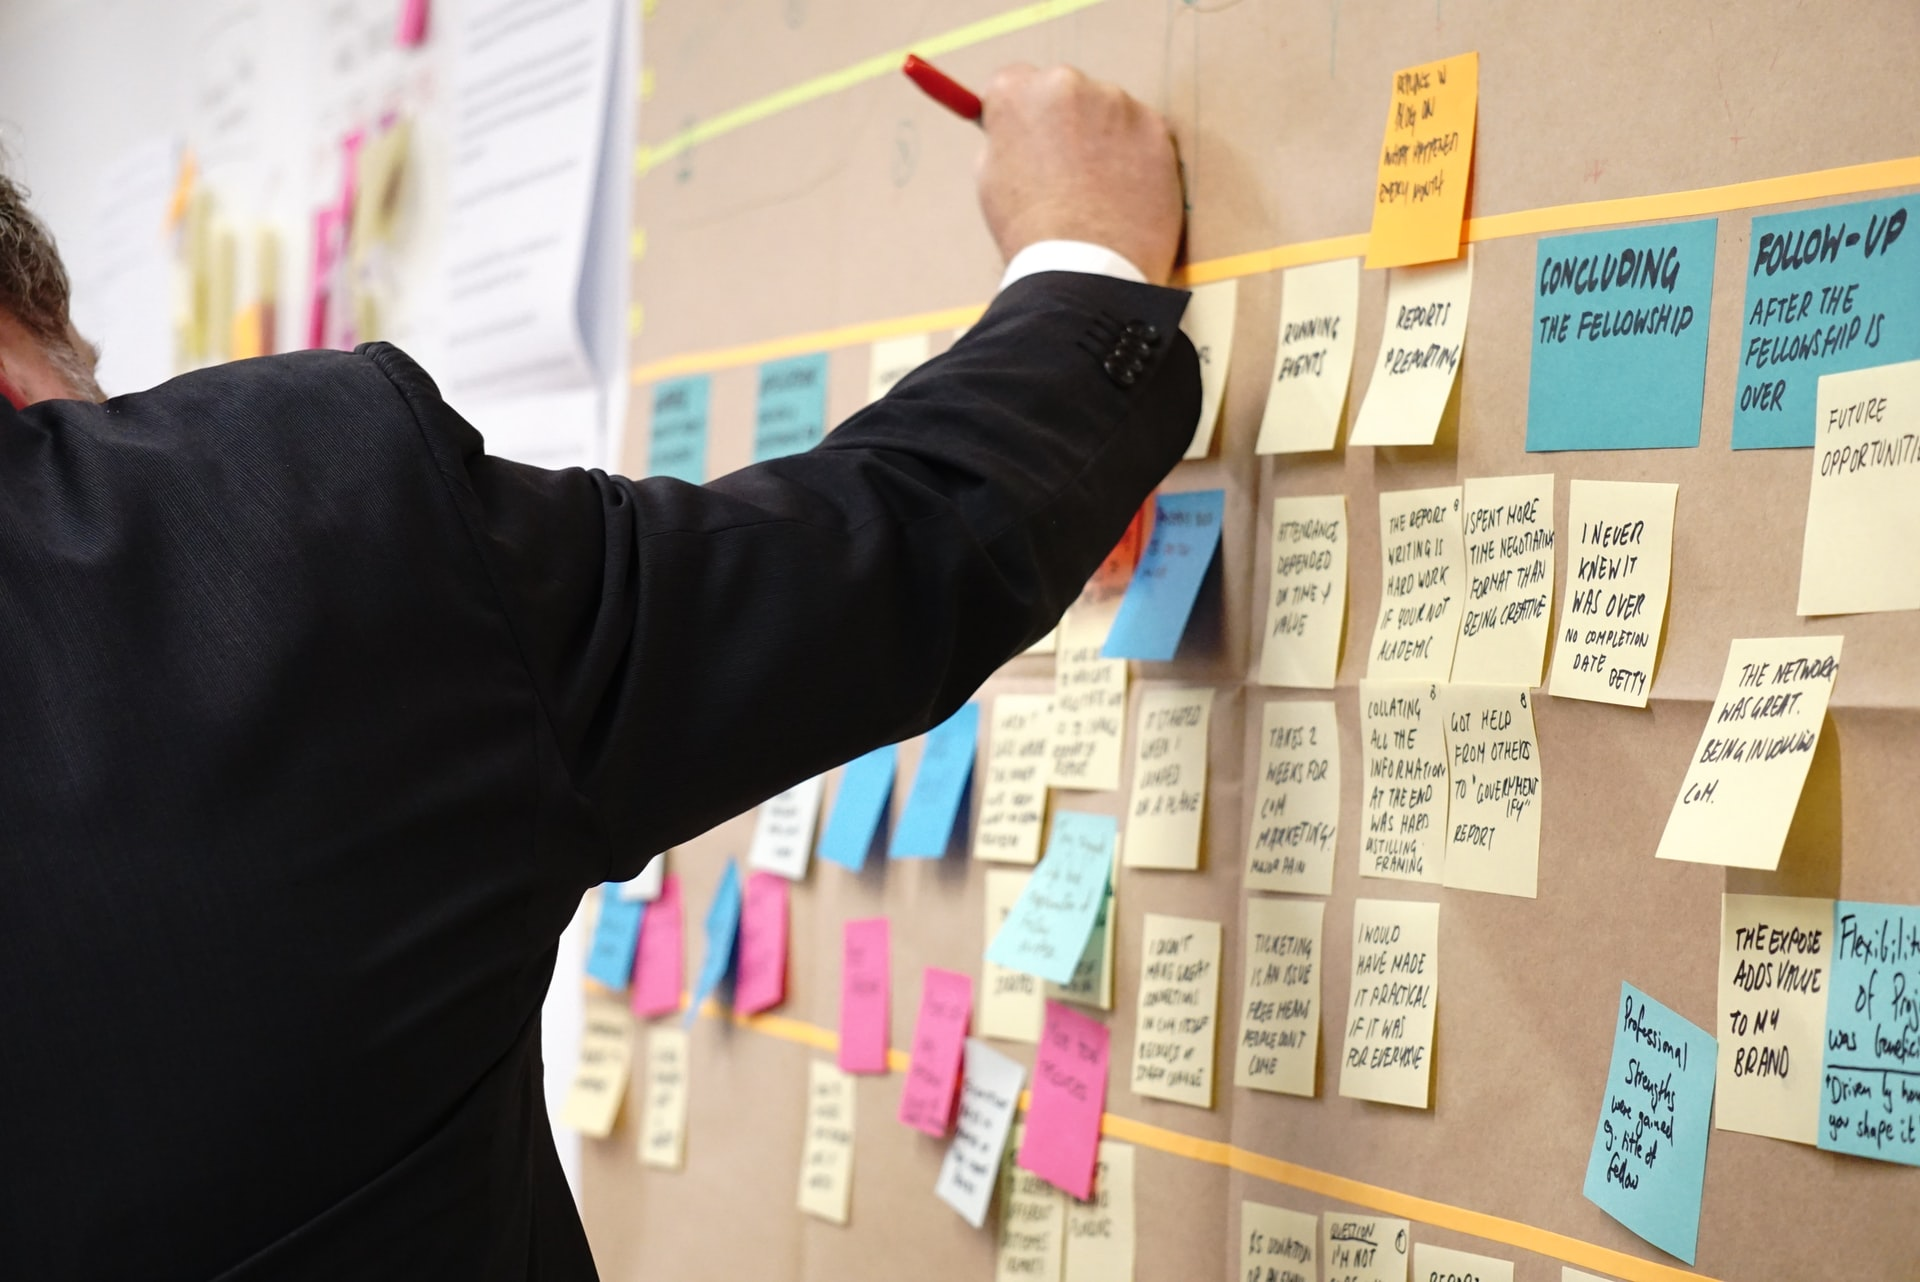
\includegraphics[width=1.1\paperwidth]{images/title.jpg}}
\end{center}
\vspace*{1cm}
{\fontsize{28}{28}\selectfont \textbf \varTitle}\\[0.35cm]
{\fontsize{20}{20}\selectfont \varSubTitle}\\[1.2cm]
{\fontsize{16}{16}\selectfont \varAuthor}\\[0.25cm]
{\fontsize{16}{16}\selectfont \varCompany}

  \newpage
  \TileWallPaper{\paperwidth}{\paperheight}{images/background.pdf}

  % see A1.3
  % see B6.3
  % generate the table of contents
  \tableofcontents

  % finish page
  \clearpage

  % use the arabic numbering system
  \pagenumbering{arabic}

  % reset page counter
  \setcounter{page}{1}

  % see B6.1a
  % create a phantom toc entry for "Umfeld und Ablauf"
  \clearpage\phantomsection\addcontentsline{toc}{part}{Umfeld und Ablauf}

  % [2]: Seite 11
\chapter{Aufgabenstellung}

Dieses Kapitel beinhaltet die komplette Aufgabenstellung im originalen Wortlaut.

\section{Ausgangslage}

\lipsum[1-2]

\section{Detaillierte Aufgabenstellung}

\lipsum[3-9]

\section{Mittel und Methoden}
\lipsum[10]
  % [2]: Seite 11
\chapter{Deklaration}

Folgender Abschnitt beschreibt die Vorkenntnisse des Kandidaten und dessen Vorbereitung.

\section{Vorkenntnisse}

\lipsum[11]

\section{Vorarbeiten}

\lipsum[12]

\section{Neue Lerninhalte}

\lipsum[13]

\section{Arbeiten in den letzten 6 Monaten}

\lipsum[14]

  % see B6.2a
\chapter{Projektaufbauorganisation}

% Diesen Abschnitt anpassen.
Das Projekt \placeholder\ wird in der Abteiltung \enquote{\varCompanyDepartment} umgesetzt. Projektleiter ist \placeholder\ und für die IPA auch die verantwortliche Fachkraft. Für die fachliche Umsetzung des hier beschriebenen Projekts ist ausschliesslich die Zusammenarbeit zwischen \placeholder\ und dem Kandidaten notwendig.

Im Unterschied zur üblichen Arbeit im Betrieb, werden zwei Experten die Arbeits des Kandidaten Begleiten und Bewerten. Die Projektaufbauorganisation ist in \ref{fig:organigram} visualisiert.

\begin{figure}[H]
  \begin{multicols}{2}
    \begin{forest}
      for tree={draw,grow'=0,folder,align=left}
      [\textbf{\varCompany}
        [\textbf{HR}
          [(BB) \\ \varVocationalTrainer]
        ]
        [...]
        [\textbf{\varCompanyDepartment}
          [(VF) \\ \varResponsibleSpecialist]
          [(K) \\ \varCandidate]
        ]
      ]
    \end{forest}

    \begin{forest}
      for tree={draw,grow'=0,folder,align=left}
      [\textbf{\varExaminationBoard}
        [\textbf{\varExaminationBoardDepartment}
          [(HEX) \\ \varPrimaryExpert]
          [(NEX) \\ \varSecondaryExpert]
        ]
      ]
    \end{forest}
  \end{multicols}
  \caption[\enquote{Organigramm der am Projekt teilnehmenden Personen} visualisiert mit TikZ Forest]{\gls{Organigramm} der am Projekt teilnehmenden Personen}
  \label{fig:organigram}
\end{figure}
  % see A1.2
% see A3
% see B6.2b
\begin{landscape}
  \chapter{Zeitplan}
  Der Zeitplan basiert auf der Vorlage \cite{Buhler_ipa-timetable_2022} und zeigt mit einer Auflösung von zwei Stundenblöcken die geplanten und getätigten Aufwände.
  \begin{figure}[H]
    \begin{center}
      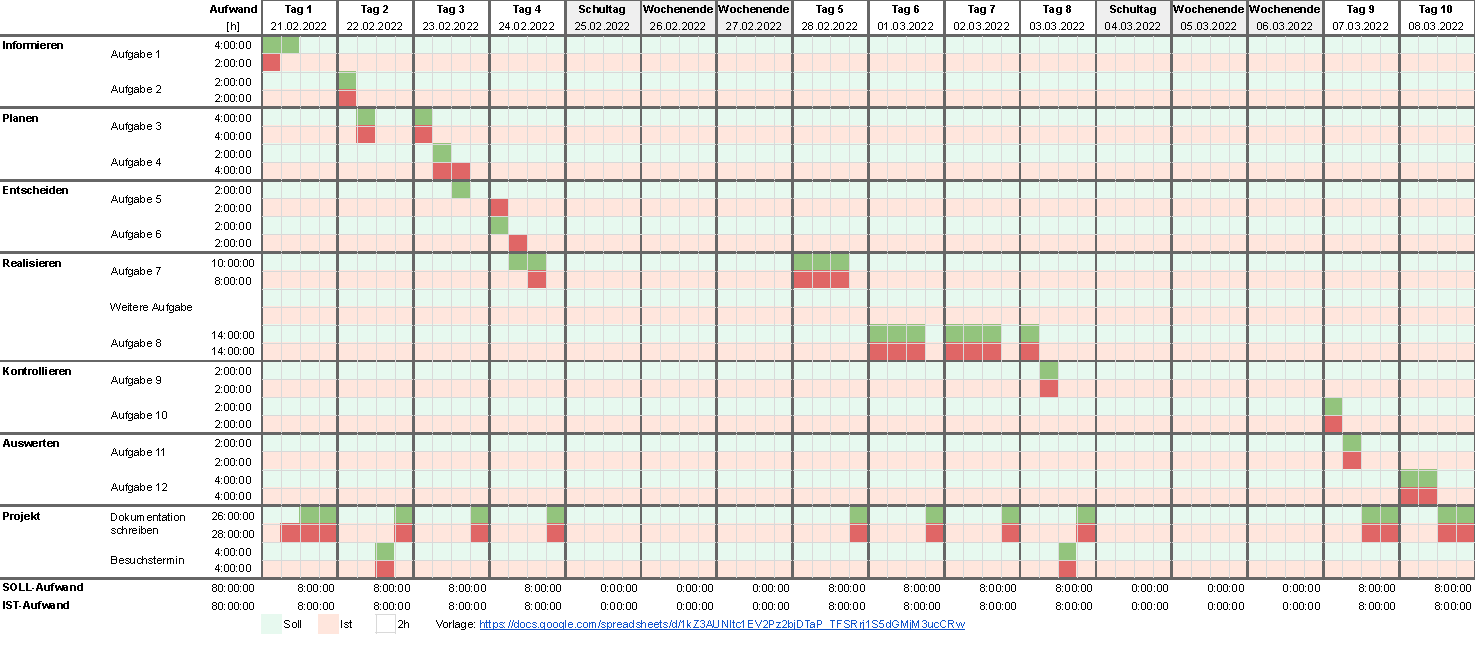
\includegraphics[width=1.55\textheight]{../res/timeplan.pdf}
    \end{center}
    \caption[\enquote{Zeitplan} erstellt mit Google Sheets]{Zeitplan}
    \label{fig:timeplan}
  \end{figure}
\end{landscape}

  % see A2.1
% see B6.2c
\chapter{Arbeitsjournal}

\section{Tag 1}
\begin{tabularx}{\textwidth}[H]{|l|X|}
  \hline
  Erledigte Arbeiten & \lipsum[23] \\ \hline
  Ungeplante Arbeiten & \lipsum[24] \\ \hline
  Erfolge & \lipsum[25] \\ \hline
  Misserfolge & \lipsum[26] \\ \hline
  Hilfestellungen & \lipsum[27] \\
  \hline
\end{tabularx}

\newpage

\section{Tag 2}
\begin{tabularx}{\textwidth}[H]{|l|X|}
  \hline
  Erledigte Arbeiten & \lipsum[23] \\ \hline
  Ungeplante Arbeiten & \lipsum[24] \\ \hline
  Erfolge & \lipsum[25] \\ \hline
  Misserfolge & \lipsum[26] \\ \hline
  Hilfestellungen & \lipsum[27] \\
  \hline
\end{tabularx}

\newpage

\section{Tag 3}
\begin{tabularx}{\textwidth}[H]{|l|X|}
  \hline
  Erledigte Arbeiten & \lipsum[23] \\ \hline
  Ungeplante Arbeiten & \lipsum[24] \\ \hline
  Erfolge & \lipsum[25] \\ \hline
  Misserfolge & \lipsum[26] \\ \hline
  Hilfestellungen & \lipsum[27] \\
  \hline
\end{tabularx}

\newpage

\section{Tag 4}
\begin{tabularx}{\textwidth}[H]{|l|X|}
  \hline
  Erledigte Arbeiten & \lipsum[23] \\ \hline
  Ungeplante Arbeiten & \lipsum[24] \\ \hline
  Erfolge & \lipsum[25] \\ \hline
  Misserfolge & \lipsum[26] \\ \hline
  Hilfestellungen & \lipsum[27] \\
  \hline
\end{tabularx}

\newpage

\section{Tag 5}
\begin{tabularx}{\textwidth}[H]{|l|X|}
  \hline
  Erledigte Arbeiten & \lipsum[23] \\ \hline
  Ungeplante Arbeiten & \lipsum[24] \\ \hline
  Erfolge & \lipsum[25] \\ \hline
  Misserfolge & \lipsum[26] \\ \hline
  Hilfestellungen & \lipsum[27] \\
  \hline
\end{tabularx}

\newpage

\section{Tag 6}
\begin{tabularx}{\textwidth}[H]{|l|X|}
  \hline
  Erledigte Arbeiten & \lipsum[23] \\ \hline
  Ungeplante Arbeiten & \lipsum[24] \\ \hline
  Erfolge & \lipsum[25] \\ \hline
  Misserfolge & \lipsum[26] \\ \hline
  Hilfestellungen & \lipsum[27] \\
  \hline
\end{tabularx}

\newpage

\section{Tag 7}
\begin{tabularx}{\textwidth}[H]{|l|X|}
  \hline
  Erledigte Arbeiten & \lipsum[23] \\ \hline
  Ungeplante Arbeiten & \lipsum[24] \\ \hline
  Erfolge & \lipsum[25] \\ \hline
  Misserfolge & \lipsum[26] \\ \hline
  Hilfestellungen & \lipsum[27] \\
  \hline
\end{tabularx}

\newpage

\section{Tag 8}
\begin{tabularx}{\textwidth}[H]{|l|X|}
  \hline
  Erledigte Arbeiten & \lipsum[23] \\ \hline
  Ungeplante Arbeiten & \lipsum[24] \\ \hline
  Erfolge & \lipsum[25] \\ \hline
  Misserfolge & \lipsum[26] \\ \hline
  Hilfestellungen & \lipsum[27] \\
  \hline
\end{tabularx}

\newpage

\section{Tag 9}
\begin{tabularx}{\textwidth}[H]{|l|X|}
  \hline
  Erledigte Arbeiten & \lipsum[23] \\ \hline
  Ungeplante Arbeiten & \lipsum[24] \\ \hline
  Erfolge & \lipsum[25] \\ \hline
  Misserfolge & \lipsum[26] \\ \hline
  Hilfestellungen & \lipsum[27] \\
  \hline
\end{tabularx}

\newpage

\section{Tag 10}
\begin{tabularx}{\textwidth}[H]{|l|X|}
  \hline
  Erledigte Arbeiten & \lipsum[23] \\ \hline
  Ungeplante Arbeiten & \lipsum[24] \\ \hline
  Erfolge & \lipsum[25] \\ \hline
  Misserfolge & \lipsum[26] \\ \hline
  Hilfestellungen & \lipsum[27] \\
  \hline
\end{tabularx}

  % see B6.1a
  % create a phantom toc entry for "Projekt"
  \clearpage\phantomsection\addcontentsline{toc}{part}{Projekt}

  % See B1
\chapter{Kurzfassung}

Die Kurzfassung gibt einen Überblick über das vorliegende Projekt.

\section{Ausgangssituation}

\lipsum[20]

\section{Umsetzung}

\lipsum[21-22]

\section{Ergebnis}

\lipsum[22]
  % see A1.1a
\chapter{Informieren}
Die nachfolgende Dokumentation baut auf der Vorlage \cite{Buhler_ipa-template_2022} auf.

\section{Fragen und Antworten}
Der Auftrag ist nicht an allen Stellen eindeutig klar. Die notwendigen Präzisierungen werden hier dokumentiert.

\begin{itemize}
  \item \textbf{Bei den Beschreibungen der Attribute im Auftrag befinden sich teilweise mehrere Begriffe für ein Attribut auf einer Zeile. Bei \texttt{Referenz, Materialien, Unterlagen} ist dies bspw. der Fall. Sind dies als einzelne, separate Datenfelder zu werten oder dienen die Begriffe auch zur Beschreibung?} Bei manchen Zeilen gibt es mehrere Begriffe, die ein einzelnes Datenfeld beschreiben. Es handelt sich aber pro Zeile um ein einzelnes Datenfeld. In der Benutzeroberfläche sollten die Begriffe angezeigt werden.
\end{itemize}

\section{Projektmanagement}
Das Projekt nach der Projektmanagementmethode IPERKA abgewickelt. Diese Methode passt zum Auftrag, weil der Auftrag in einer Iteration innerhalb von 10 Tagen wasserfallartig realisiert werden soll.

\subsection{Arbeitspakete}
Der Auftrag kann ich folgende Arbeitspakete aufgeteilt und nach den Phasen der Projektmanagementmethode gegliedert werden:

\begin{itemize}
    \item Informieren
    \begin{description}
        \item[AP1: Anforderungen analysieren] Der Auftrag wird analysiert und daraus einzelne Arbeitspakete abgeleitet. 
        \item[AP2: Lorem] \lipsum[2][1]
    \end{description}
    \item Planen
    \begin{description}
        \item[AP3: Lorem] \lipsum[2][2] 
        \item[AP4: Lorem] \lipsum[2][3]
    \end{description}
    \item Entscheiden
    \begin{description}
        \item[AP5: Lorem] \lipsum[2][4] 
        \item[AP6: Lorem] \lipsum[2][5]
    \end{description}
    \item Realisieren
    \begin{description}
        \item[AP7: Lorem] \lipsum[2][6] 
        \item[AP8: Lorem] \lipsum[2][7]
    \end{description}
    \item Kontrollieren
    \begin{description}
        \item[AP9: Lorem] \lipsum[2][8] 
        \item[AP10: Lorem] \lipsum[2][9]
    \end{description}
    \item Auswerten
    \begin{description}
        \item[AP11: Lorem] \lipsum[2][10] 
        \item[AP12: Lorem] \lipsum[2][11]
    \end{description}
\end{itemize}

\section{Systemaufbau}
Im Folgenden wird die Einbettung des Systems in das Gesamtsystem gezeigt, sowie die vorhandenen Schnittstellen und Akteure beschrieben.

\subsection{Gesamtsystem}

\subsection{Schnittstellen}

\subsection{Akteure}
  % see A1.4
\chapter{Planen}

Die Zeitplanung wird in der Abbildung \ref{fig:timeplan} oberhalb gezeigt. Die restlichen Aspekte der Planung sind in diesem Kapitel dokumentiert.

\section{Anwendungsfälle}

\section{Testkonzept}
Das Testkonzept beschreibt, wie und mit welchen Werkzeugen das Resultat auf seine Richtigkeit kontrolliert wird.

\subsection{Testmethoden}

\subsection{Testmittel}
  \chapter{Entscheiden}
Dieses Kapitel beschreibt, welche Entscheide wie getroffen wurden.

\section{Sprache der Bezeichner}
Der Auftrag gibt ein Datenmodell vor, wobei die einzelnen Bezeichner im Auftrag in Deutsch beschrieben sind. Da es üblich ist, dass Programmcode in Englisch verfasst wird, werden auch diese Bezeichner, wie Segment, Startzeitpunkt oder Änderungsdatum im Code und in der Planung übersetzt und so verwendet.
  \chapter{Realisieren}
  \chapter{Kontrollieren}
  \chapter{Auswerten}

  % see B6.6
  % create a phantom toc entry for the index/glossary table
  \clearpage\phantomsection\addcontentsline{toc}{part}{Glossar}

  % generate glossary
  \printnoidxglossary[title={Glossar}]

  % create a phantom toc entry for the figures table
  \clearpage\phantomsection\addcontentsline{toc}{part}{Abbildungsverzeichnis}

  % generate figures table
  \listoffigures

  % create a phantom toc entry for the literature table
  \clearpage\phantomsection\addcontentsline{toc}{part}{Literaturverzeichnis}

  % generate bibliography
  \printbibliography[title=Literaturverzeichnis]

  % defines the beginning of the appendix
  \appendix

  % create a phantom toc entry for "Projekt"
  \clearpage\phantomsection\addcontentsline{toc}{part}{Anhang}

  % see B6.1b
\chapter{Quellcode}

\begin{figure}[H]
  \begin{codebox}[]
    \begin{minted}{javascript}
/**
 * @param {number} maxNumber
 * @return {number[]}
 */
 export default function sieveOfEratosthenes(maxNumber) {
  const isPrime = new Array(maxNumber + 1).fill(true);
  isPrime[0] = false;
  isPrime[1] = false;

  const primes = [];

  for (let number = 2; number <= maxNumber; number += 1) {
    if (isPrime[number] === true) {
      primes.push(number);

      /*
       * Optimisation.
       * Start marking multiples of `p` from `p * p`, and not from `2 * p`.
       * The reason why this works is because, at that point, smaller multiples
       * of `p` will have already been marked `false`.
       *
       * Warning: When working with really big numbers, the following line may cause overflow
       * In that case, it can be changed to:
       * let nextNumber = 2 * number;
       */
      let nextNumber = number * number;

      while (nextNumber <= maxNumber) {
        isPrime[nextNumber] = false;
        nextNumber += number;
      }
    }
  }

  return primes;
}
    \end{minted}
  \end{codebox}
  \caption[\enquote{Sieb des Eratosthenes implementiert mit JavaScript} visualisiert mit Minted]{Sieb des Eratosthenes implementiert mit JavaScript}
  \label{fig:sieve-of-eratosthenes}
\end{figure}

\end{document}
